\chapter[The association between tumour spatial structure and clinical diagnostics]{The association between tumour spatial structures and clinical diagnostics or subtype classification}
\label{Chap:4}	%CREATE YOUR OWN LABEL.
\pagestyle{headings}
\label{Sec:4.1_intro}	%CREATE YOUR OWN LABEL.
\section{Introduction}
The variability of cell organisations across tumour microenvironments (TMEs) and patients is the central issue that hinders successful anti-cancer treatment. Spatially, TMEs are often diversely organised and constantly change in response to external stimulations (i.e. chemotherapy, radiotherapy) which ultimately assist these cells’ survival and metastasis to neighbouring organisms \cite{wu2022spatial}. Studies have shown that TMEs are shaped and coordinated by the crosstalk between cancer cells to facilitate the development of cancer \cite{jin2020updated, quail2013microenvironmental, schurch2020coordinated}. TMEs and cancer-immune cell communication are regarded as two complex mechanisms in cancer that are arising as a potential target for cancer therapy, especially targeted therapy and immunotherapy \cite{jin2020updated, abou2020integrating, qiu2017reprogramming}. Experimental and computational approaches are highly desirable to properly understand the heterogeneity and mutability of the TMEs across multiple samples and cancer subtypes. 

The distribution of the cells in spatial context can be the result of the crosstalk between cancer and immune cells \cite{van2018spatially}. As discussed in Chapters \ref{Chap:2} and \ref{Chap:3}, the advances in multiplexing spatial transcriptomic and proteomic (spatial-omic) experimental technologies have enabled us to uncover the spatial structure of the TMEs at an unprecedented resolution and throughput capacity. It is anticipated that the ultimate spatial tumour atlas for uncovering the variation across cancer subtypes and/or patients \cite{wu2022spatial} will emerge as a contemporary research approach. The combination of multimodal analysis including spatial transcriptomic, proteomic and molecular measurements can result in a holistic description of the state of cancer for each patient \cite{boehm2022harnessing}. It is often seen that spatial-omics data are collected in large quantities and generated in multiple batches. There are several analysis frameworks for spatial data quantification have been developed (discussed in Chapters \ref{Chap:Intro}). However, there is a limited number of computational frameworks have been reported to be able to perform multimodal spatial-omic data integration. 
% \begin{enumerate}
%     \item Perform registration to seamlessly align multiple adjacent images
%     \item Integrate data 
%     \item Facilitate high-res image display and interactive data exploration through Napari
%     \item Perform tissue heterogeneity analysis across multiple ROIs/FOVs
%     \item Export/Import single-cell analysis result to visualisation
% \end{enumerate}

In this chapter, I developed an interactive analysis package called Multi-Omics Spatial Analysis Platform (MOSAP) with a focus on data integration from multiple spatial-omic data and identification of the variations in spatial heterogeneity. MOSAP is implemented to address three key challenges of multimodal analysis and multi-samples analysis power. Firstly, MOSAP provides a function to seamlessly register images from multiple adjacent tissue sections. While high throughput experiments for spatial transcriptomic and proteomic are extensively developing, a single platform that works for both types of spatial-mic data is not yet ready. Therefore, the experiment is often performed by using multiple adjacent tissue sections with each section used as the sample for a single spatial-omic data. Secondly,                


% of cell populations in cancer exhibit considerable diversity in both inter-tumour and intra-tumour heterogeneity. The diversity
% The tumour microenvironment is a dynamic ecosystem with diverse cells self-organise and complex networks of the cell-cell neighbourhood. From chapter \ref{Chap:3}, I presented the analysis results of using cell communities as the representation of different regions within the tissue. In this chapter, I aim to develop quantitative computation approaches to infer differences between different cancer subtypes and clinical outcomes.     
\section{MOSAP - MultiOmics Spatial Analysis Platform}
\subsection{The structure of MOSAP}
\begin{figure}
    \centering
    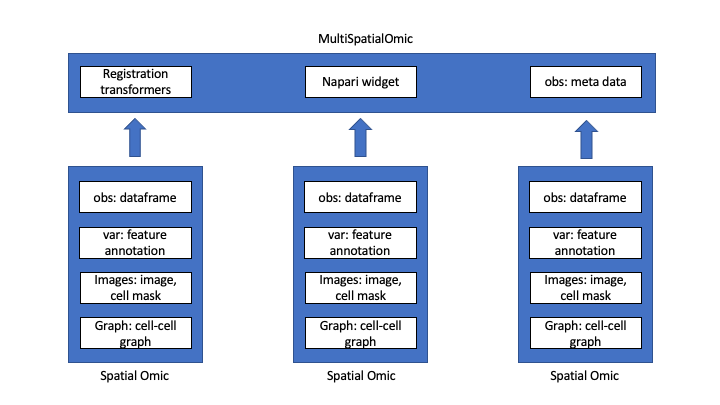
\includegraphics[width=0.8\columnwidth]{Chapter4/Figures/Chap4_MOSAP_OOP.png}
    \caption[Schematic drawing of the SpatialOmic objects as the building block of MOSAP]{Schematic drawing of the SpatialOmic objects as the building block of MOSAP}
    \label{Chap4:MOSAP_OOP}
\end{figure}
MOSAP is implemented 
\subsection{Registration of images from adjacent tissue sections}
The rise of spatial-omic technologies, including spatial transcriptomics and spatial proteomics, has created the need for a platform that can perform integrative analysis across different spatial data types. The multimodal experiments are usually performed in adjacent tissue sections which introduce variation to the tissue morphology. Therefore, image registration is often required to align the tissue from multiple rounds of experiments before any integrative analysis can be done.  

\subsection{Capability to differentiate the cell-cell interaction across conditions or cancer subtypes}
% \subsection{MOSAP methods and software}
% MOSAP is an analysis package for processing single-cell spatial-omic data designed to work with multiple samples/images. The key functionalities of MOSAP include: 


\subsubsection{The statistical model of MOSAP}
\section{Interactivly data exploration and visualisation}
In recent years, a number of graphical user interface (GUI) open-source packages specialised for multiplexed imaging have been developed. These open-source packages allow users to contribute to the analysis power through plugins, scripts, or pipelines \cite{bankhead2017qupath,schneider2012nih}.  
\section{Application of MOSAP on identifying the heterogeneity of tumour microenvironment structures in skin cancer}

The spatial distribution of cancer cells in skin cancer has distinct enrichment patterns across different subtypes including BCC, SCC, and melanoma. 

% \subsection{The variation of tumour heterogeneity across skin cancer subtypes}

For this analysis, single-cell spatial imaging of SCC, BCC and melanoma using CosMx platform. As mentioned in \ref{Chap:Intro}, CosMx is a platform for spatial transcriptomics at single-cell resolution. While the number of transcripts is currently capped at 960 genes, CosMx technology is already one of the highest throughput FISH. Additionally, the sub-cellular resolution of CosMx technology allows us to retain the location of individual RNA molecules. We generated CosMx data using three SCC, two BCC and four melanoma samples. Each tissue biopsy was selected for multiple fields of view (FOVs) and underwent the CosMX ISH.  

In collaboration with a team member, the cell type of CosMx was projected from scRNA-seq data (Figure \ref{Chap4:fig1}A). Next, MOSAP is applied to perform heterogeneity across the FOVs using cell type information. By applying Delaunay triangulation to cell spatial coordinates, a network of cell-cell neighbourhood networks is constructed. We applied Rao’s quadratic entropy to each cell in the network to measure the diversity of connection between the observing cell and neighboring cells (i.e. two cells sharing an edge). Using Rao’s quadratic entropy scoring as a measurement for heterogeneity has two advantages. First, the entropy score considers both the probability of two neighbouring cells (i.e. two cells sharing an edge) being different cell types. Second, Rao’s quadratic entropy also considers spatial distance between each member of the neighbouring pair, which is important for cell-cell interaction through paracrine signalling. Each cell in the network was scored by the diversity of its connections, and these scores were visualised as a heatmap (Figure \ref{Chap4:fig1}B). FOV 15 from SCC patient B18 had the highest overall entropy score and was selected for further exploration of the factors contributing to the overall heterogeneity. The regions of this FOV that exhibited a high level of heterogeneity were enriched for immune cell types including B cells, plasmacytoid dendritic cells (pDCs), and myeloid and T cells (Figure \ref{Chap4:fig1}A). Voronoi diagram mapping of cell communities indicated spatial domains composed of different groups of cell types. We identified eight distinct cell communities in FOV 15, including one (Community 7) showing a high density of immune cells consistent with our heterogeneity heatmap (Figure \ref{Chap4:fig1}B, C).  

To compare cell type heterogeneity across the different skin cancer subtypes, we grouped scores across all FOVs by cancer type, and detected a significant increase in cell type heterogeneity score in the melanoma samples compared to in NMSC (Figure \ref{Chap4:fig1}D). This finding indicates that the cellular microenvironment in melanoma skin contains a wider variety of cell types coexisting than is seen in other skin cancers.

\begin{figure}
    \centering
    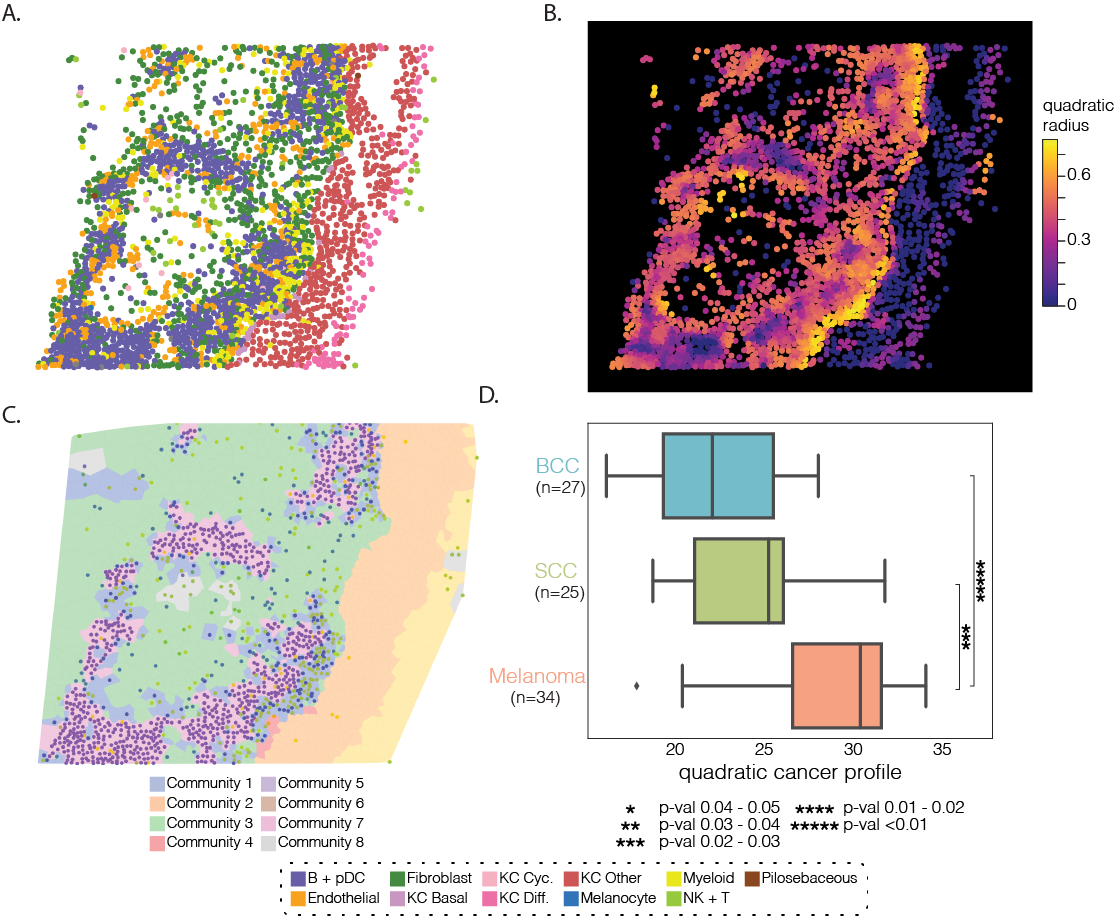
\includegraphics[width=0.8\columnwidth]{Chapter4/Figures/Chap4_figure_2.png}
    \caption[The spatial heterogeneity analysis across the skin cancer subtype]{The spatial heterogeneity analysis across the skin cancer subtype. (A, B) The cell type annotation using CosMx data of patient B18 and the heatmap of the spatial cell heterogeneity from the same FOV. (C) Voronoi diagram of eight cell communities identified in the tissue shown in (A-B) and cell types overlaying of community 7 (pink). (D) Boxplot of heterogeneity scores across three skin cancer types, indicating the greatest overall heterogeneity score for melanoma.)}
    \label{Chap4:fig1}
    
\end{figure}

% Here we measured the variation of different cell types population from multiple FOVs across the patient tissues to find spatial patterns enrich for each skin cancer subtypes, (2) the gene markers that enrich specific communities. 

% A potential approach to cancer marker screening 
% \subsection{Conserved tumor microenvironment communities across skin patient samples}
% Result with the comparison of cell type across multiple Polaris, CosMx images 

\section{The tumour microenvironment analysis across patients in colorectal cancer samples}

This is work in progress. For this work, we will perform the correlation analysis of pairwise distance between every cell type and clinical outcome. 

We performed network construction using Delaunay triangulation across 170 ROIs and filtered out the pair of distance that larger than 40 $\mu$m as a threshold for cell to be communication through paracrine. The results showed that the fold change of distance between immune cells (B-cell, NK-cell ) in close neighborhood is highly associated to MSI alteration and casualty (Figure \ref{Chap4:fig2})

Using cell-cell distance as a feature to predict clinical outcome and genomic status

\subsection{TME variation as a potential predictive model for clinical outcome}
\begin{figure}
    \centering
    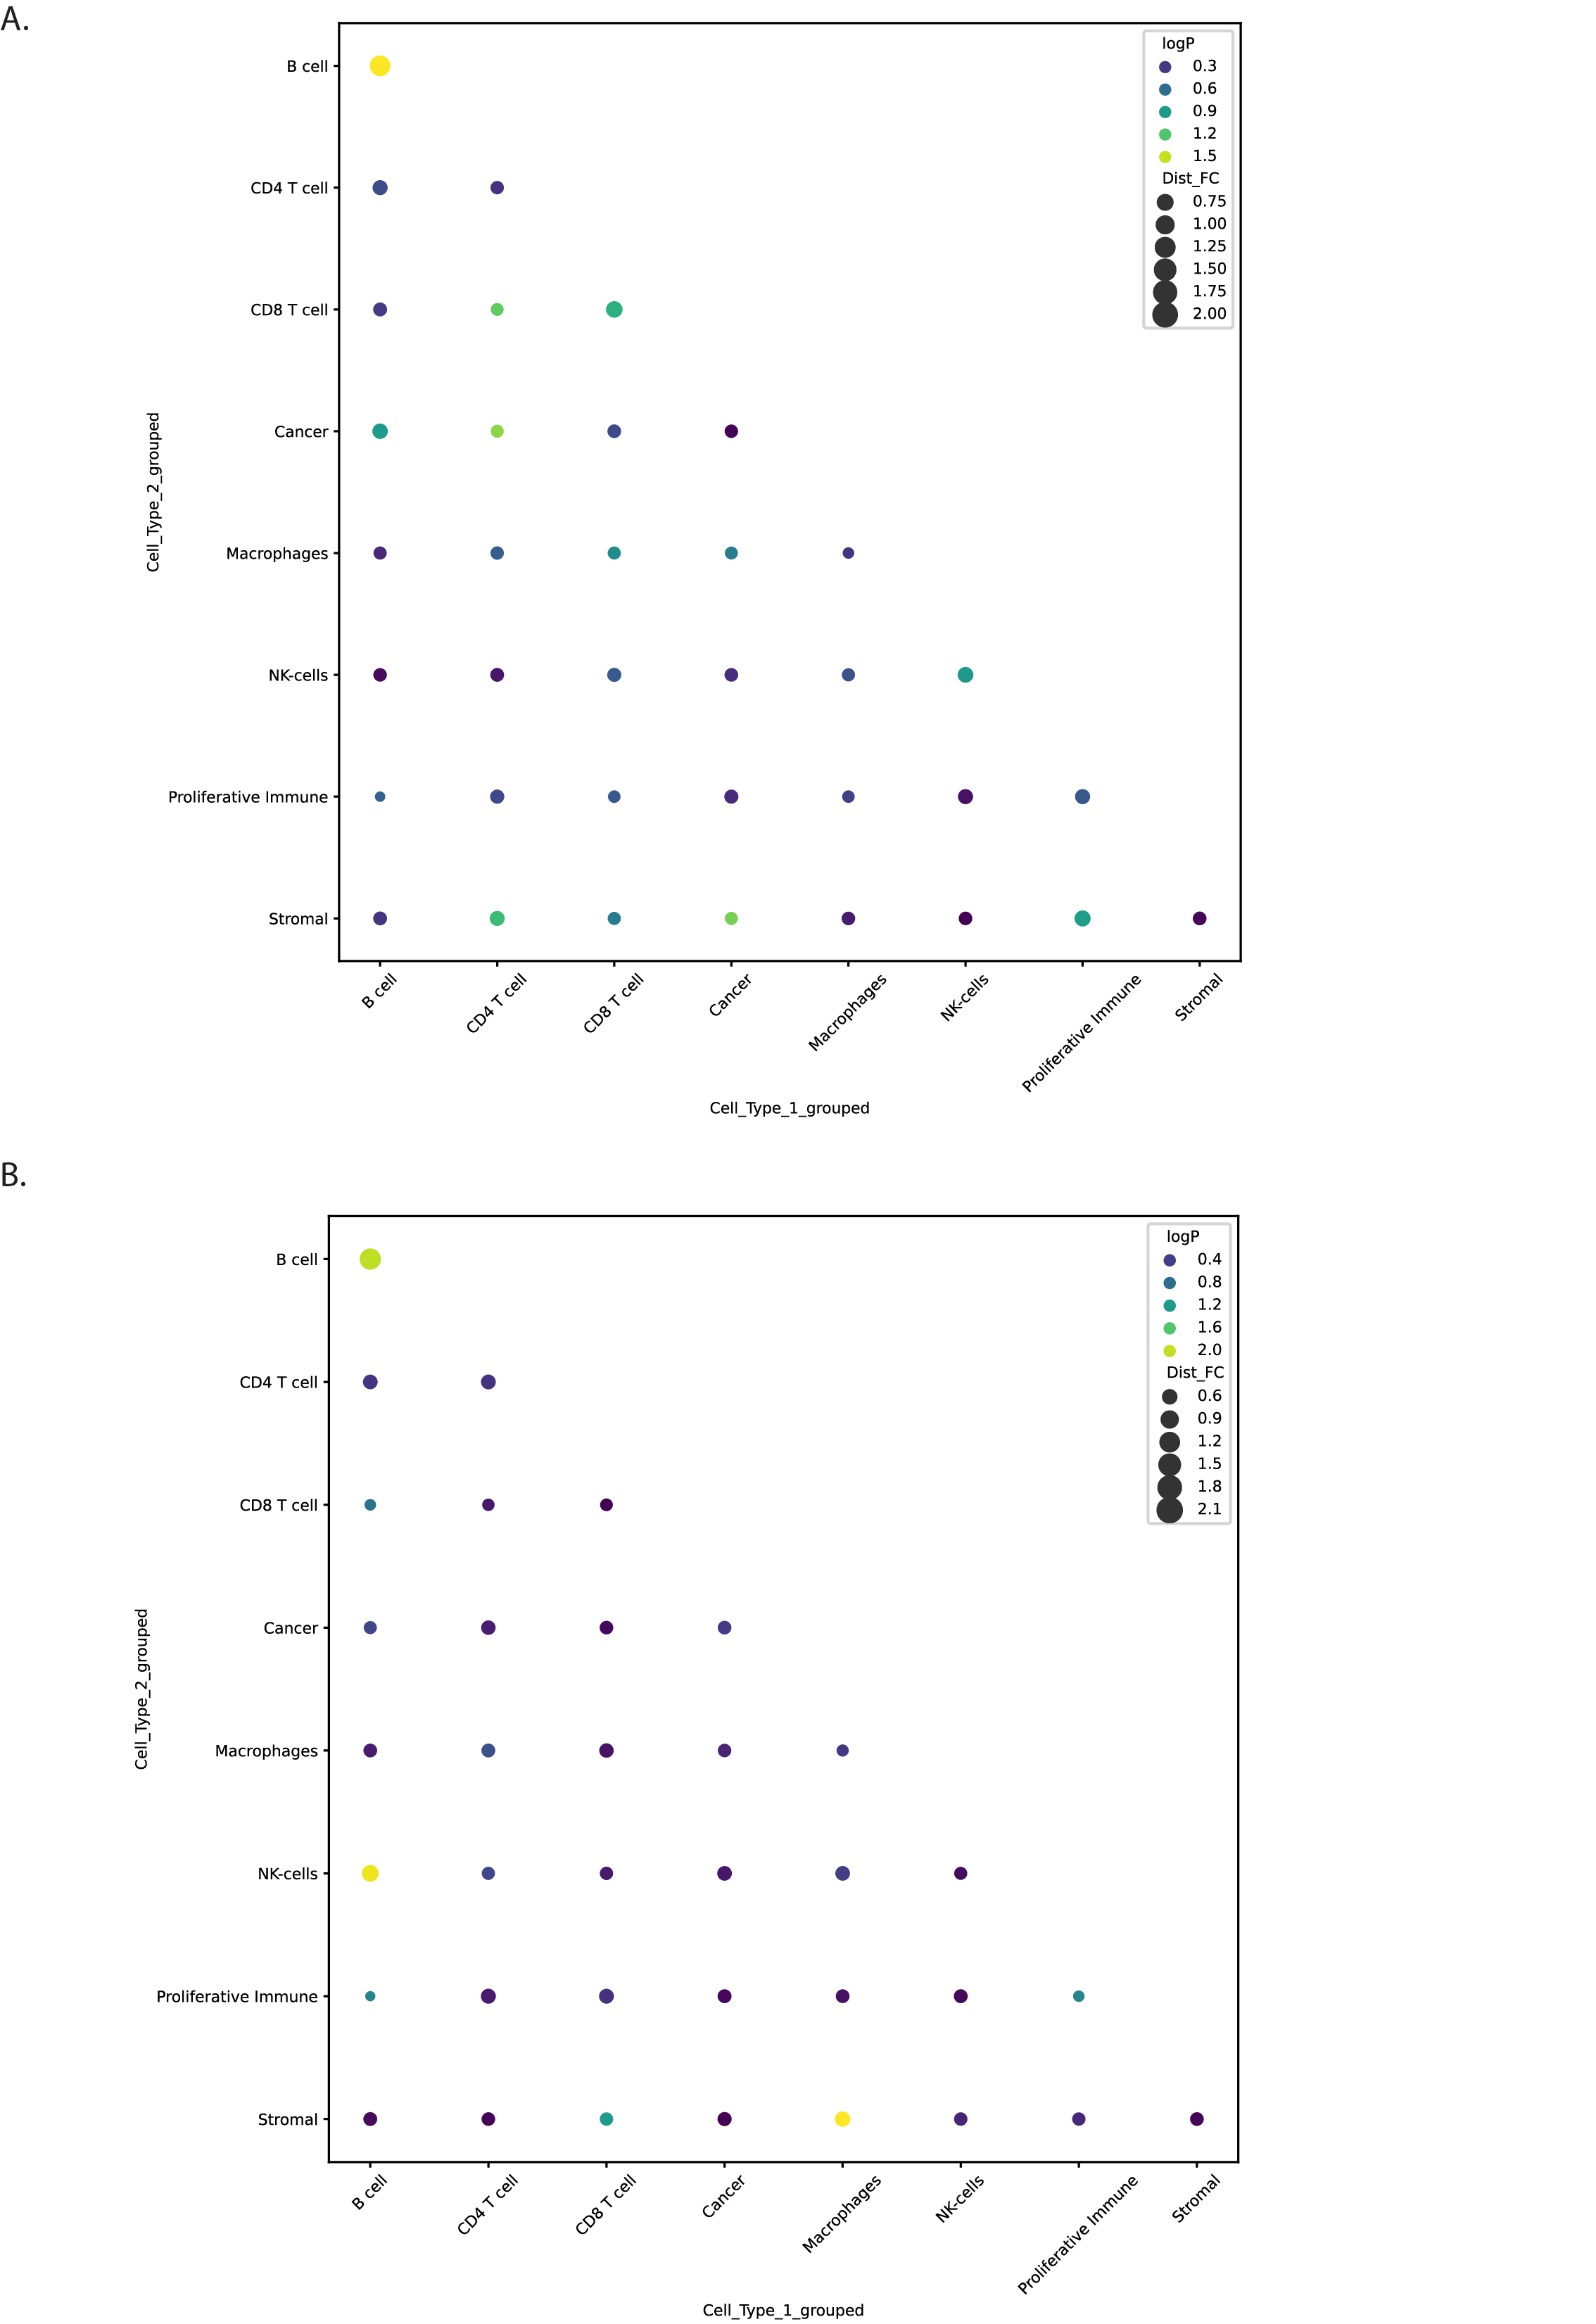
\includegraphics[width=0.8\columnwidth]{Chapter4/Figures/Chap4_figure1.png}
    \caption[The association of cell-cell interaction with the genomic status and clinical outcome]{The association of cell-cell interaction with the genomic status and clinical outcome. (A) The correlation of cell-cell interaction and the MSI status of the colorectal cancer dataset. (B) The correlation of cell-cell interaction and the clinical outcome (long and short survival)}
    \label{Chap4:fig2}
    
\end{figure}
% % \label{Sec:4.2_Cell_communities}	%CREATE YOUR OWN LABEL.
% \subsection{The correlation of genomic features and cell types neighborhood}
% \subsection{The spatial features of cell-cell interaction as predictive model of survival rates}
% ********* Enter your text below this line: ********

% ***************************************************


% ***************************************************
% \section{}
% \label{Sec:4.3_quantitative_validation}	%CREATE YOUR OWN LABEL.
% \subsection{}
% ********* Enter your text below this line: ********

% ***************************************************
% \bibliographystyle{elsarticle-num}

% \bibliography{./References/Bibliography}